\chapter{Introduction}
\label{chapter:introduction}

% adapted widely: \cite{ResoJachalskyRosenhahnOstermann:2013, LiuTuzelRamalingamChellappa:2011, LevinshteinStereKutulakosFleetDickinsonSiddiqi:2009, AchantaShajiSmithLucchiFuaSuesstrunk:2010}
The term superpixel was introduced by Ren and Malik in 2003 \cite{RenMalik:2003} and is used to describe a group of pixels similar in color or other low-level features. The concept of superpixels is motivated by two important aspects, which have been adapted widely. Firstly, pixels do not represent natural entities but are merely a result of discretization~\cite{RenMalik:2003}. And secondly, the number of pixels prevents many algorithms from being feasible \cite{RenMalik:2003}. At this point, Ren and Malik introduce superpixels as more natural entities -- grouping pixels which perceptually belong together\footnote{Of course, ``perceptually belong[ing] together'', or ``perceptually meaningful'' as Veksler \etal~\cite{VekslerBoykovMehrani:2010} put it, cannot be used as mathematical definition. Mostly this refers to similarity in color and spatial consistency \cite{VekslerBoykovMehrani:2010}.}.
% TODO: maybe mention superpixel as atomic region

% superpixel segmentation = oversegmentation:  \cite{HuazhuFuXiaochunCaoDaiTangYahongHanDongXu:2014, DaiTangHuazhaFuXiaochunCao:2012, MoorePrinceWarrellMohammedJones:2008, VanDenBerghBoixRoigCapitaniVanGool:2012, RenMalik:2003, WeikersdorferGossowBeetz:2012}
% recent algorithms: \cite{HuazhuFuXiaochunCaoDaiTangYahongHanDongXu:2014, DaiTangHuazhaFuXiaochunCao:2012, MoorePrinceWarrellMohammedJones:2008, VanDenBerghBoixRoigCapitaniVanGool:2012, AchantaShajiSmithLucchiFuaSuesstrunk:2010, LiuTuzelRamalingamChellappa:2011, LevinshteinStereKutulakosFleetDickinsonSiddiqi:2009, VekslerBoykovMehrani:2010, ZhangHartleyMashfordBurn:2011, ConradMertzMester:2013, DaiTangHuazhaFuXiaochunCao:2012, PerbetStengerMaki:2012, WeikersdorferGossowBeetz:2012}
% not intended for superpixel segmentation: \cite{FelzenswalbHuttenlocher:2004, ShiMalik:2000, VedaldiSoatto:2008}
The task of segmenting an image into superpixels is widely referred to as oversegmentation or superpixel segmentation. While recent algorithms are explicitly designed to generate superpixel segmentations, others were initially intended for classical image segmentation or clustering. Overall, superpixels may have different properties which first of all impose a visual difference. Figure \ref{fig:introduction-running-examples} presents the running examples of this thesis, each image oversegmented using a different superpixel algorithm.
\begin{figure}
	\centering
	\subfigure{
		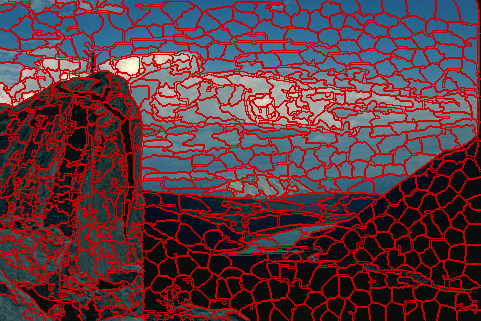
\includegraphics[scale=\scalefivebsd]{pictures/bsd-1-seeds-revised-spatial-mean-pixels}
	}
	\subfigure{
		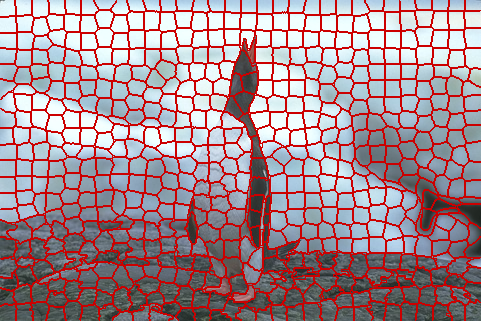
\includegraphics[scale=\scalefivebsd]{pictures/bsd-2-slic}
	}
	\subfigure{
		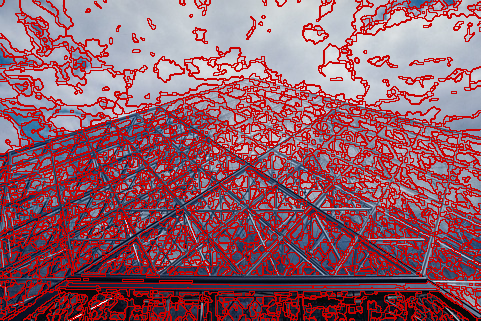
\includegraphics[scale=\scalefivebsd]{pictures/bsd-3-fh}
	}
	\subfigure{
		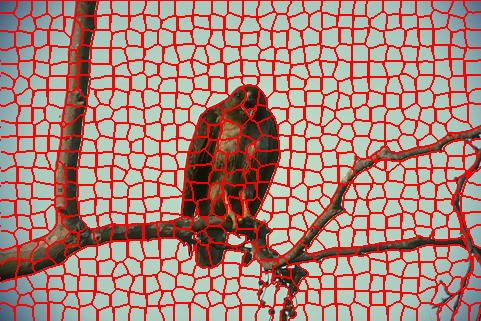
\includegraphics[scale=\scalefivebsd]{pictures/bsd-4-tp}
	}
	\subfigure{
		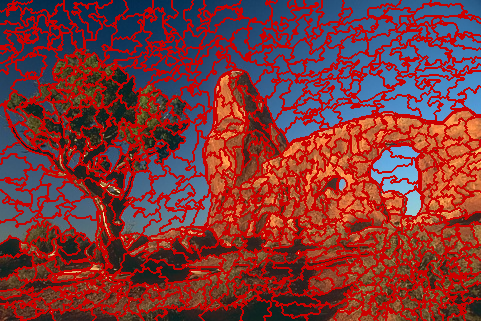
\includegraphics[scale=\scalefivebsd]{pictures/bsd-5-ers}
	}
	\subfigure{
		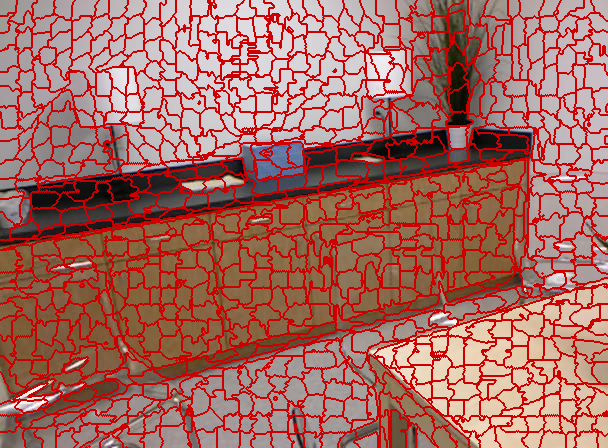
\includegraphics[scale=\scalefivenyu]{pictures/nyu-1-crs}
	}
	\subfigure{
		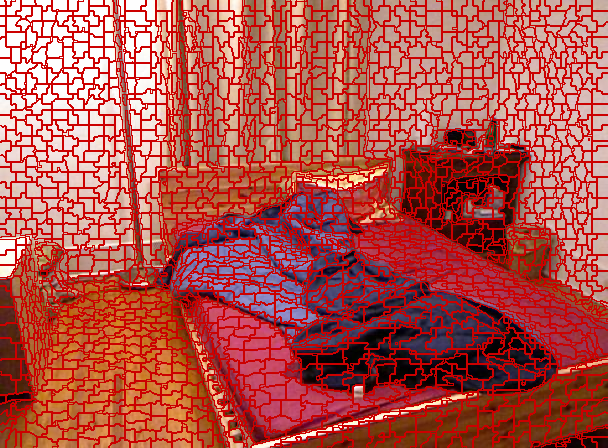
\includegraphics[scale=\scalefivenyu]{pictures/nyu-2-vccs}
	}
	\subfigure{
		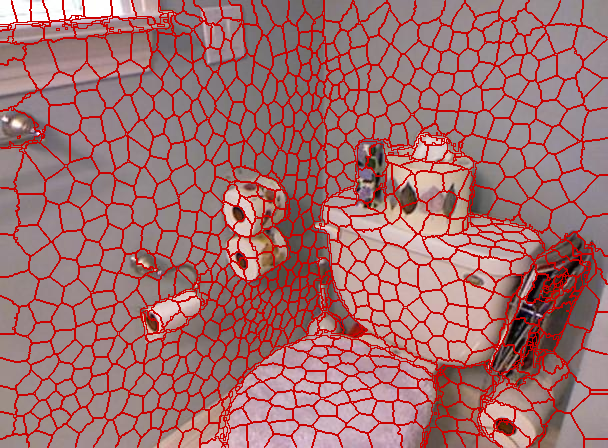
\includegraphics[scale=\scalefivenyu]{pictures/nyu-3-dasp}
	}
	\subfigure{
		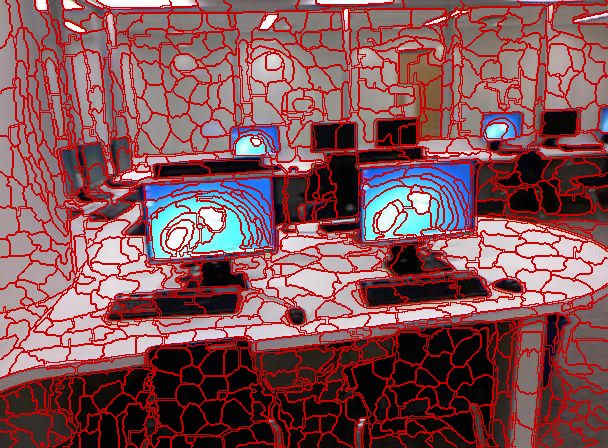
\includegraphics[scale=\scalefivenyu]{pictures/nyu-4-seeds3d}
	}
	\subfigure{
		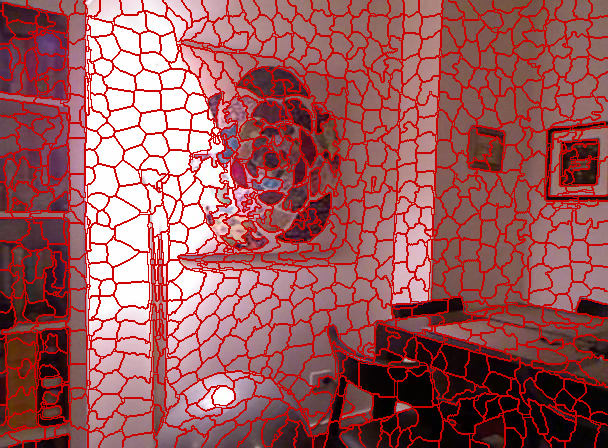
\includegraphics[scale=\scalefivenyu]{pictures/nyu-5-slic3d}
	}
	\caption[The running examples of this thesis taken from the Berkeley Segmentation Dataset \cite{ArbelaezMaireFowlkesMalik:2011} and the NYU Depth Dataset \cite{SilbermanHoiemKohliFergus:2012}.]{The running examples of this thesis will be used to introduce and evaluate several superpixel algorithms. Top: images taken from the Berkeley Segmentation Dataset \cite{ArbelaezMaireFowlkesMalik:2011} oversegmented into roughly $600$ superpixels. Bottom: images taken from the NYU Depth Dataset \cite{SilbermanHoiemKohliFergus:2012} oversegmented into roughly $840$ superpixels.}
	\label{fig:introduction-running-examples}
\end{figure}

% applications: \cite{ShuWangHuchuanLuFanYangMingHsuanYang:2011, FanYangHuchuanLuMingHsuanYang:2014, YuhangZhangHartleyMashfordBurn:2011, JainTuragaBriggmanHelmstadterDenkSeung:2011, GuptaArbelaezMalik:2013, RenMalik:2003, TigheLazebnik:2010, VanDenBerghRoigBoixManenVanGool:2013}
% algorithms: \cite{AchantaShajiSmithLucchiFuaSuesstrunk:2010, LiuTuzelRamalingamChellappa:2011, LevinshteinStereKutulakosFleetDickinsonSiddiqi:2009, MoorePrinceWarrellMohammedJones:2008, MoorePrinceWarrell:2010, VekslerBoykovMehrani:2010, ZengWangWangGanZha:2011, ZhangHartleyMashfordBurn:2011, VanDenBerghBoixRoigCapitaniVanGool:2012, WeikersdorferGossowBeetz:2012, PaponAbramovSchoelerWoergoetter:2013, ConradMertzMester:2013, DaiTangHuazhaFuXiaochunCao:2012, PerbetStengerMaki:2012, SivaWong:2014, RohkohlEngel:2007, DruckerMacCormick:2009}
Since their introduction, superpixels have actively been used for a wide range of applications: for example as pre-processing step for classical segmentation \cite{RenMalik:2003,RohkohlEngel:2007}, as mid-level cues used for tracking \cite{ShuWangHuchuanLuFanYangMingHsuanYang:2011}, as pre-processing step for graph-based stereo matching \cite{YuhangZhangHartleyMashfordBurn:2011}, or for semantic segmentation \cite{GuptaArbelaezMalik:2013}. In addition, numerous superpixel algorithms have been proposed. Although it may depend on the application which of these algorithms is preferable, most authors agree on the following basic requirements for superpixels \cite{LevinshteinStereKutulakosFleetDickinsonSiddiqi:2009,AchantaShajiSmithLucchiFuaSuesstrunk:2010,LiuTuzelRamalingamChellappa:2011}:
\begin{itemize}
	\item Superpixels should respect object boundaries;
	\item Superpixels should be generated as efficiently as possible;
	\item Superpixels should not lower the achievable performance\footnote{Here and in the following, performance refers to the quality of a superpixel segmentation rather than its runtime.} of subsequent processing steps.
\end{itemize}
Additional requirements may include compactness, especially in regions where no object boundaries are present \cite{LevinshteinStereKutulakosFleetDickinsonSiddiqi:2009,SchickFischerStiefelhagen:2012}, as well as connectivity \cite{LevinshteinStereKutulakosFleetDickinsonSiddiqi:2009}.

% video superpixels: \cite{AchantaShajiSmithLucchiFuaSuesstrunk:2012, ResoJachalskyRosenhahnOstermann:2013, ChangDonglaiWeiFisher:2013, HuazhuFuXiaochunCaoDaiTangYahongHanDongXu:2014, VanDenBerghRoigBoixManenVanGool:2013}
Until 2012, superpixel algorithms were designed to oversegment images with respect to the requirements stated above. However, with rising availability of low-cost RGB-D cameras, algorithms utilizing depth information become increasingly interesting for applications. Furthermore, extending the idea of superpixel segmentation to the temporal domain of videos is receiving increased attention. Approaches using depth information to oversegment videos \cite{WeikersdorferSchickCremers:2013} have recently been proposed. While some superpixel algorithms can naturally be extended to depth or video data, others may be constrained to color images or need to be adapted. One of the latter, although easily generalized to process video data \cite{VanDenBerghRoigBoixManenVanGool:2013}, is the approach proposed by Van den Bergh \etal \cite{VanDenBerghBoixRoigCapitaniVanGool:2012}, called \textbf{SEEDS}\footnote{\textbf{SEEDS} stands for ``Superpixels Extracted via Energy-Driven Sampling'' \cite{VanDenBerghBoixRoigCapitaniVanGool:2012}, see chapter \ref{chapter:superpixel-segmentation} for details.}. As \textbf{SEEDS} represents a superpixel algorithm showing both excellent runtime as well as state-of-the-art performance, the focus of this thesis lies in integrating depth information into \textbf{SEEDS}. Our goal is to preserve the low runtime while increasing performance by utilizing depth information.

% Another focus of this thesis is of comparative nature. Despite of the daunting number of superpixel algorithms available, only few research is devoted to comparing and analyzing the different approaches within a consistent framework: \cite{SchickFischerStiefelhagen:2012, NeubertProtzel:2012} and \cite{AchantaShajiSmithLucchiFuaSuesstrunk:2012}. While suitable datasets as for example the Berkeley Segmentation Dataset \cite{ArbelaezMaireFowlkesMalik:2011} or the NYU Depth Dataset \cite{SilbermanHoiemKohliFergus:2012} are available, used evaluation measures, as for example the Undersegmentation Error, are not defined consistently \cite{NeubertProtzel:2012, AchantaShajiSmithLucchiFuaSuesstrunk:2012} and implementations are mostly not made publicly available to reproduce the results presented in the corresponding publications. Another important aspect to consider, although this may seem trivial, is the availability of implementations for different platforms. Most algorithms are implemented using MatLab or C/C++ using a wide range of different libraries. Often the actual implementations differ from the proposed algorithm, as for example \textbf{SEEDS}, or details concerning the implementation are not discussed in detail. Therefore, it is difficult to determine both the state-of-the-art as well as algorithms suited for specific applications.

Another focus of this thesis lies in a comparative assessment of all superpixel algorithms providing source code. We find this necessary as only few research is devoted to comparing and evaluating the rising number of approaches within a consistent framework. To the best of our knowledge these are \cite{SchickFischerStiefelhagen:2012, NeubertProtzel:2012} and \cite{AchantaShajiSmithLucchiFuaSuesstrunk:2012}. We base our experiments on both the Berkeley Segmentation Dataset \cite{ArbelaezMaireFowlkesMalik:2011} as well as the NYU Depth Dataset \cite{SilbermanHoiemKohliFergus:2012}. While the Berkeley Segmentation Dataset is commonly used to assess superpixel algorithms, performance on the NYU Depth Dataset may be of particular interest for specific applications. In particular, the scenes captured by the NYU Depth Dataset provide a fresh contrast to the natural images from the Berkeley Segmentation Dataset. Additionally, it provides depth images allowing us to evaluate additional algorithms requiring depth information. Furthermore, widely used evaluation measures are not defined consistently throughout the literature, as for example the Undersegmentation Error \cite{NeubertProtzel:2012, AchantaShajiSmithLucchiFuaSuesstrunk:2012}. Another commonly used measure is Boundary Recall \cite{MartinFowlkesMalik:2004}. However, evaluation based on these two measures only may give a highly biased impression such that an assessment using additional measures is necessary. Finally, details concerning the available implementations, as well as the parameter selection is often omitted within the corresponding publications. Overall, it is difficult to determine both the state-of-the-art as well as approaches suited for specific applications. In our opinion, this is highly unsatisfactory.

\section{Contributions}

The main contributions of this thesis are:~
\begin{itemize}
	\item An implementation of \textbf{SEEDS} including a variant providing a compactness parameter \cite{VanDenBerghBoixRoigVanGool:2013} and several extensions utilizing depth information.
	\item A thorough evaluation of several superpixel algorithms on the Berkeley Segmentation Dataset and the NYU Depth Dataset using an extended version of the Berkeley Segmentation Benchmark providing additional measures to evaluate superpixel algorithms.
\end{itemize}
The extended Berkeley Segmentation Benchmark is made publicly available together with our implementation of \textbf{SEEDS}.

\section{Outline}

The thesis is organized as follows: After this short introduction, chapter \ref{chapter:related-work} reviews the literature on superpixel algorithms. Chapter \ref{chapter:superpixel-segmentation} gives a thorough introduction to \textbf{SEEDS} as well as another superpixel algorithm used as baseline, called \textbf{SLIC}\footnote{\textbf{SLIC} stands for ``Simple Linear Iterative Clustering'', see chapter \ref{chapter:related-work} for details.}~\cite{AchantaShajiSmithLucchiFuaSuesstrunk:2010}. Then, chapter \ref{chapter:superpixel-segmentation-depth} discusses several approaches to superpixel segmentation utilizing depth information. This includes a detailed discussion of integrating depth information into \textbf{SLIC}. Chapter \ref{chapter:seeds-depth} represents the main part of this thesis and discusses several extensions of \textbf{SEEDS} to depth. We present several variants of \textbf{SEEDS} using depth information and focus on two of them for evaluation. The datasets and measures used for evaluation are discussed in chapter \ref{chapter:datasets}. Chapter \ref{chapter:evaluation} presents experimental results of several superpixel algorithms. Parameters are optimized individually on training/validation sets before the different algorithms are compared on the corresponding test sets with regard to their qualitative and quantitative performance as well as runtime. Chapter \ref{chapter:conclusion} gives a short conclusion, a brief outlook and presents ideas for future work in this area.

% The appendix includes documentation of the Berkeley Segmentation Benchmark, as we found that the benchmark lacks detailed documentation, the Extended Berkeley Segmentation Benchmark as well as further tables and figures concerning the qualitative and quantitative comparison given in chapter \ref{chapter:evaluation}.

%\section{Nomenclature}
%
%We use the term \textit{superpixel algorithm}\index{superpixel algorithm} to denote an algorithm generating an oversegmentation of a RGB or RGB-D image. The terms \textit{oversegmentation} and \textit{superpixel segmentation} are used interchangeably. The terms \textit{supervoxel} and \textit{temporal supervoxel}, as introduced in chapter \ref{chapter:related-work}, are used to denote a segmentation of a point cloud and a video sequence, respectively. The term \textit{superpixel} always denotes a single, connected segment within a superpixel segmentation. The same goes for supervoxel and temporal supervoxel in their respective domains.